% Credits are indicated where needed. The general idea is based on a template by Vel (vel@LaTeXTemplates.com) and Frits Wenneker.

\documentclass[11pt, a4paper]{article} % General settings in the beginning (defines the document class of your paper)
% 11pt = is the font size
% A4 is the paper size
% “article” is your document class

%----------------------------------------------------------------------------------------
%	Packages
%----------------------------------------------------------------------------------------

% Necessary
\usepackage[german,english]{babel} % English and German language 
\usepackage{booktabs} % Horizontal rules in tables 
% For generating tables, use “LaTeX” online generator (https://www.tablesgenerator.com)
\usepackage{placeins}
\usepackage{comment} % Necessary to comment several paragraphs at once
\usepackage[utf8]{inputenc} % Required for international characters
\usepackage[T1]{fontenc} % Required for output font encoding for international characters

% Might be helpful
\usepackage{amsmath,amsfonts,amsthm} % Math packages which might be useful for equations
\usepackage{tikz} % For tikz figures (to draw arrow diagrams, see a guide how to use them)
\usepackage{tikz-cd}
\usetikzlibrary{positioning,arrows} % Adding libraries for arrows
\usetikzlibrary{decorations.pathreplacing} % Adding libraries for decorations and paths
\usepackage{tikzsymbols} % For amazing symbols ;) https://mirror.hmc.edu/ctan/graphics/pgf/contrib/tikzsymbols/tikzsymbols.pdf 
\usepackage{blindtext} % To add some blind text in your paper
\usepackage{subcaption} % For subfigure environment
\usepackage{hyperref}

%---------------------------------------------------------------------------------
% Additional settings
%---------------------------------------------------------------------------------
\usepackage{indentfirst} 
%---------------------------------------------------------------------------------
% Define your margins
\usepackage{geometry} % Necessary package for defining margins

\geometry{
	top=2cm, % Defines top margin
	bottom=2cm, % Defines bottom margin
	left=2.2cm, % Defines left margin
	right=2.2cm, % Defines right margin
	includehead, % Includes space for a header
	%includefoot, % Includes space for a footer
	%showframe, % Uncomment if you want to show how it looks on the page 
}

\setlength{\parindent}{15pt} % Adjust to set you indent globally 

%---------------------------------------------------------------------------------
% Define your spacing
\usepackage{setspace} % Required for spacing
% Two options:
\linespread{1.5}
%\onehalfspacing % one-half-spacing linespread

%----------------------------------------------------------------------------------------
% Define your fonts
\usepackage[T1]{fontenc} % Output font encoding for international characters
\usepackage[utf8]{inputenc} % Required for inputting international characters

\usepackage{XCharter} % Use the XCharter font


%---------------------------------------------------------------------------------
% Define your headers and footers

\usepackage{fancyhdr} % Package is needed to define header and footer
\pagestyle{fancy} % Allows you to customize the headers and footers
\setlength{\headheight}{13.59999pt} % Adjust head height to avoid fancyhdr warning

%\renewcommand{\sectionmark}[1]{\markboth{#1}{}} % Removes the section number from the header when \leftmark is used

% Headers
\lhead{STAT 333} % Define left header
\chead{\textit{}} % Define center header - e.g. add your paper title
\rhead{Regression Runner} % Define right header

% Footers
\lfoot{} % Define left footer
\cfoot{\footnotesize \thepage} % Define center footer
\rfoot{ } % Define right footer

%---------------------------------------------------------------------------------
%	Add information on bibliography
\usepackage{natbib} % Use natbib for citing
\usepackage{har2nat} % Allows to use harvard package with natbib https://mirror.reismil.ch/CTAN/macros/latex/contrib/har2nat/har2nat.pdf

% For citing with natbib, you may want to use this reference sheet: 
% http://merkel.texture.rocks/Latex/natbib.php

%---------------------------------------------------------------------------------
% Add field for signature (Reference: https://tex.stackexchange.com/questions/35942/how-to-create-a-signature-date-page)
\newcommand{\signature}[2][5cm]{%
  \begin{tabular}{@{}p{#1}@{}}
    #2 \\[2\normalbaselineskip] \hrule \\[0pt]
    {\small \textit{Signature}} \\[2\normalbaselineskip] \hrule \\[0pt]
    {\small \textit{Place, Date}}
  \end{tabular}
}
%---------------------------------------------------------------------------------
%	General information
%---------------------------------------------------------------------------------
\title{title \thanks{The whole project is published in this \href{https://github.com/S-tanley/STAT-333-UW-Madison}{repo}}} % Adds your title
\author{
Stanley Zheng \space Eric \space Lucas
% Add your first and last name
    \thanks{Equal contribution} % Adds a footnote to your title
    %\institution{YOUR INSTITUTION} % Adds your institution
  }

\date{\small \today} % Adds the current date to your “cover” page; leave empty if you do not want to add a date


%---------------------------------------------------------------------------------
%	Define what’s in your document
%---------------------------------------------------------------------------------

\begin{document}


% If you want a cover page, uncomment "%---------------------------------------------------------------------------------
% Cover page
%---------------------------------------------------------------------------------

% Here are more templates for other cover pages: https://www.latextemplates.com/cat/title-pages

% This example is based on this cover page example: https://www.latextemplates.com/template/academic-title-page

\begin{titlepage} % Starts new environment where the page number is not displayed and the count starts at 1 for the next page

%------------------------------------------------
%	Institutional information
%------------------------------------------------
	
\begin{minipage}{0.4\textwidth} % Begins new environment (like a text box)
    \begin{flushleft} % Sets environment on the left side of the paper
    \large
    University of XX\\ % Add your institution
    Chair of Political Science IV\\ % Add the chair
    Fall 2018\\ % Add term
    COURSE TITLE\\ % Add course title
    Supervisor: NAME % Add instructor/supervisor name 
    \end{flushleft}
\end{minipage}
	
\vspace*{2in} % Adds some space in-between
	
\center % Centre everything on the page

%------------------------------------------------
%	Main part
%------------------------------------------------
	
{\huge\bfseries 值jij}\\[0.4cm] % Add your paper title 
{\large\today}\\[0.4cm] % Add date (current day)
FIRSTNAME LASTNAME % Add your name
	
\vfill % Adds additional space

%------------------------------------------------
%	General information about the author
%------------------------------------------------

\vfill % Adds additional space

Your contact info \\ % Add your contact info
Your Program \\ % Add info about your program
Semester you are enrolled \\ % Add info about your semester

\vfill % Adds additional space

%------------------------------------------------
%	Word count
%------------------------------------------------

\vfill % Adds additional space
	
Word count: XXXX % To indicate the word count
% How to check words in a LaTeX document: https://www.overleaf.com/help/85-is-there-a-way-to-run-a-word-count-that-doesnt-include-latex-commands
	

	
\end{titlepage}" and uncomment "\begin{comment}" and "\end{comment}" to comment the following lines
%%---------------------------------------------------------------------------------
% Cover page
%---------------------------------------------------------------------------------

% Here are more templates for other cover pages: https://www.latextemplates.com/cat/title-pages

% This example is based on this cover page example: https://www.latextemplates.com/template/academic-title-page

\begin{titlepage} % Starts new environment where the page number is not displayed and the count starts at 1 for the next page

%------------------------------------------------
%	Institutional information
%------------------------------------------------
	
\begin{minipage}{0.4\textwidth} % Begins new environment (like a text box)
    \begin{flushleft} % Sets environment on the left side of the paper
    \large
    University of XX\\ % Add your institution
    Chair of Political Science IV\\ % Add the chair
    Fall 2018\\ % Add term
    COURSE TITLE\\ % Add course title
    Supervisor: NAME % Add instructor/supervisor name 
    \end{flushleft}
\end{minipage}
	
\vspace*{2in} % Adds some space in-between
	
\center % Centre everything on the page

%------------------------------------------------
%	Main part
%------------------------------------------------
	
{\huge\bfseries 值jij}\\[0.4cm] % Add your paper title 
{\large\today}\\[0.4cm] % Add date (current day)
FIRSTNAME LASTNAME % Add your name
	
\vfill % Adds additional space

%------------------------------------------------
%	General information about the author
%------------------------------------------------

\vfill % Adds additional space

Your contact info \\ % Add your contact info
Your Program \\ % Add info about your program
Semester you are enrolled \\ % Add info about your semester

\vfill % Adds additional space

%------------------------------------------------
%	Word count
%------------------------------------------------

\vfill % Adds additional space
	
Word count: XXXX % To indicate the word count
% How to check words in a LaTeX document: https://www.overleaf.com/help/85-is-there-a-way-to-run-a-word-count-that-doesnt-include-latex-commands
	

	
\end{titlepage}

%\begin{comment}
\maketitle % Print your title, author name and date; comment if you want a cover page 

% \begin{center} % Center text
%     Word count: XXXX
% % How to check words in a LaTeX document: https://www.overleaf.com/help/85-is-there-a-way-to-run-a-word-count-that-doesnt-include-latex-commands
% \end{center}
%\end{comment}

%----------------------------------------------------------------------------------------
% Abstract
%----------------------------------------------------------------------------------------
\setcounter{page}{1} % Sets counter of page to 1
%----------------------------------------------------------------------------------------
% Introduction
%----------------------------------------------------------------------------------------

\section{Introduction} % Main section title

\subsection{Motivation: The Shifting Landscape of the NBA} % Sub-section 1.1
% Paragraph 1: General observation and the basic rule
Over the last couple of decades, anyone watching the NBA has noticed a big change in how the game is played. We see teams shooting 
way more three-pointers than before. It makes sense to ask why. In the NBA, the basic rule is that shots made inside the arc are 
worth 2 points, while shots made further out, behind the arc, are worth 3 points. This simple difference in scoring value seems to 
have encouraged teams to focus more and more on shooting from distance.

% Paragraph 2: The "Three-Point Era" narrative and motivation for study
This trend is so noticeable that people often talk about the modern NBA as the "Three-Point Era". Famous players like Stephen Curry 
really showed how valuable long-range shooting can be, making teams rethink their strategies. But is this just a popular trend, or 
has the actual importance of making three-pointers for winning games really increased compared to the past? For teams trying to win 
championships, understanding if and how the value of different shots has changed is really important. In today's world with lots of 
data available, we felt that using statistical analysis could help quantify this change and maybe offer useful insights for teams 
trying to optimize how they play.

\subsection{Research Question and Approach} % Sub-section 1.2
% Paragraph 1: Core question and the "story"

So, the main question we wanted to investigate in this project is: How has the \textbf{statistical association} between key shooting 
metrics, especially three-point percentage (3P\%), and team success, measured by win rate, changed over the last approximately 
15-20 years? Our "story" is essentially testing the common idea that the NBA has truly entered a "three-point era" where making 
threes is more strongly linked to winning than it used to be.

% Paragraph 2: Challenge and approach
We need to be careful, though. We are using data collected from watching games (observational data), not from a controlled 
experiment like an RCT (Randomized Controlled Trial). This means we can't easily prove that shooting more threes \textbf{causes} more 
wins, because many other things might be happening at the same time (like better players, different defenses, rule changes). So, 
our approach is to use statistical tools to look for strong patterns or \textbf{structural evidence} in the data that show if the association between 3P\% and winning has really 
changed significantly over time, while trying to account for some other factors. Our goal is to describe this change accurately 
based on the statistics, aiming for an interpretation that acknowledges these limitations but points towards the changing dynamics 
(a quasi-causal goal).

\subsection{Thesis Statement} % Sub-section 1.3
% Paragraph 1: Presenting the thesis
Using data comparing the 2005-2009 and 2020-2024 NBA regular seasons (source: NBA API \href{https://github.com/swar/nba_api}{https://github.com/swar/nba\_api}), we find the statistical association between 
three-point percentage (3P\%) and win rate differs significantly between these periods: NBA team-seasons (unit of analysis) in 
the 2020-2024 period with higher 3P\% also have statistically significant higher win rates, while NBA team-seasons in the 2005-2009 
period did not have statistically significant higher win rates, even after controlling for two-point efficiency and shot selection 
proportions.

%----------------------------------------------------------------------------------------
% End of Introduction Section
%----------------------------------------------------------------------------------------

%----------------------------------------------------------------------------------------
% Data Analysis
%----------------------------------------------------------------------------------------

\section{Methods}
\subsection{Dataset}
Our dataset is sourced from the \href{https://github.com/swar/nba_api}{NBA's public API}, an online interface that provides comprehensive 
and standardized statistics for teams and players across multiple seasons. The NBA API offers detailed 
data covering a wide range of performance categories, including shooting statistics, rebounding, passing, 
turnovers, fouls, player efficiency metrics, and advanced team analytics.

For our analysis, we primarily focus on shooting-related metrics, including three-point field goal percentage (3P\%), 
two-point field goal percentage (2P\%), three-point attempt rate (3PA rate), and two-point attempt rate (2PA rate). 
Even from the original dataset, 

To motivate our investigation into how the impact of three-point shooting on team success has evolved, 
we begin by comparing data from the 2005-2009 and 2020-2024 NBA regular seasons using two sets of visualizations.

% The first set of histograms(Figure \ref{fig:3P_shooting_percent}) shows the three-point shooting percentage (3P\%), capturing efficiency on three-point attempts. While the 
% distributions for the two periods overlap significantly, there is a modest rightward shift, indicating that teams have become slightly 
% more accurate from beyond the arc over time. This suggests that the increase in three-point volume has not come at the expense of efficiency, 
% but rather, teams have adapted by developing better shooters and improving shot quality.

\begin{figure}[htbp]
    \centering
    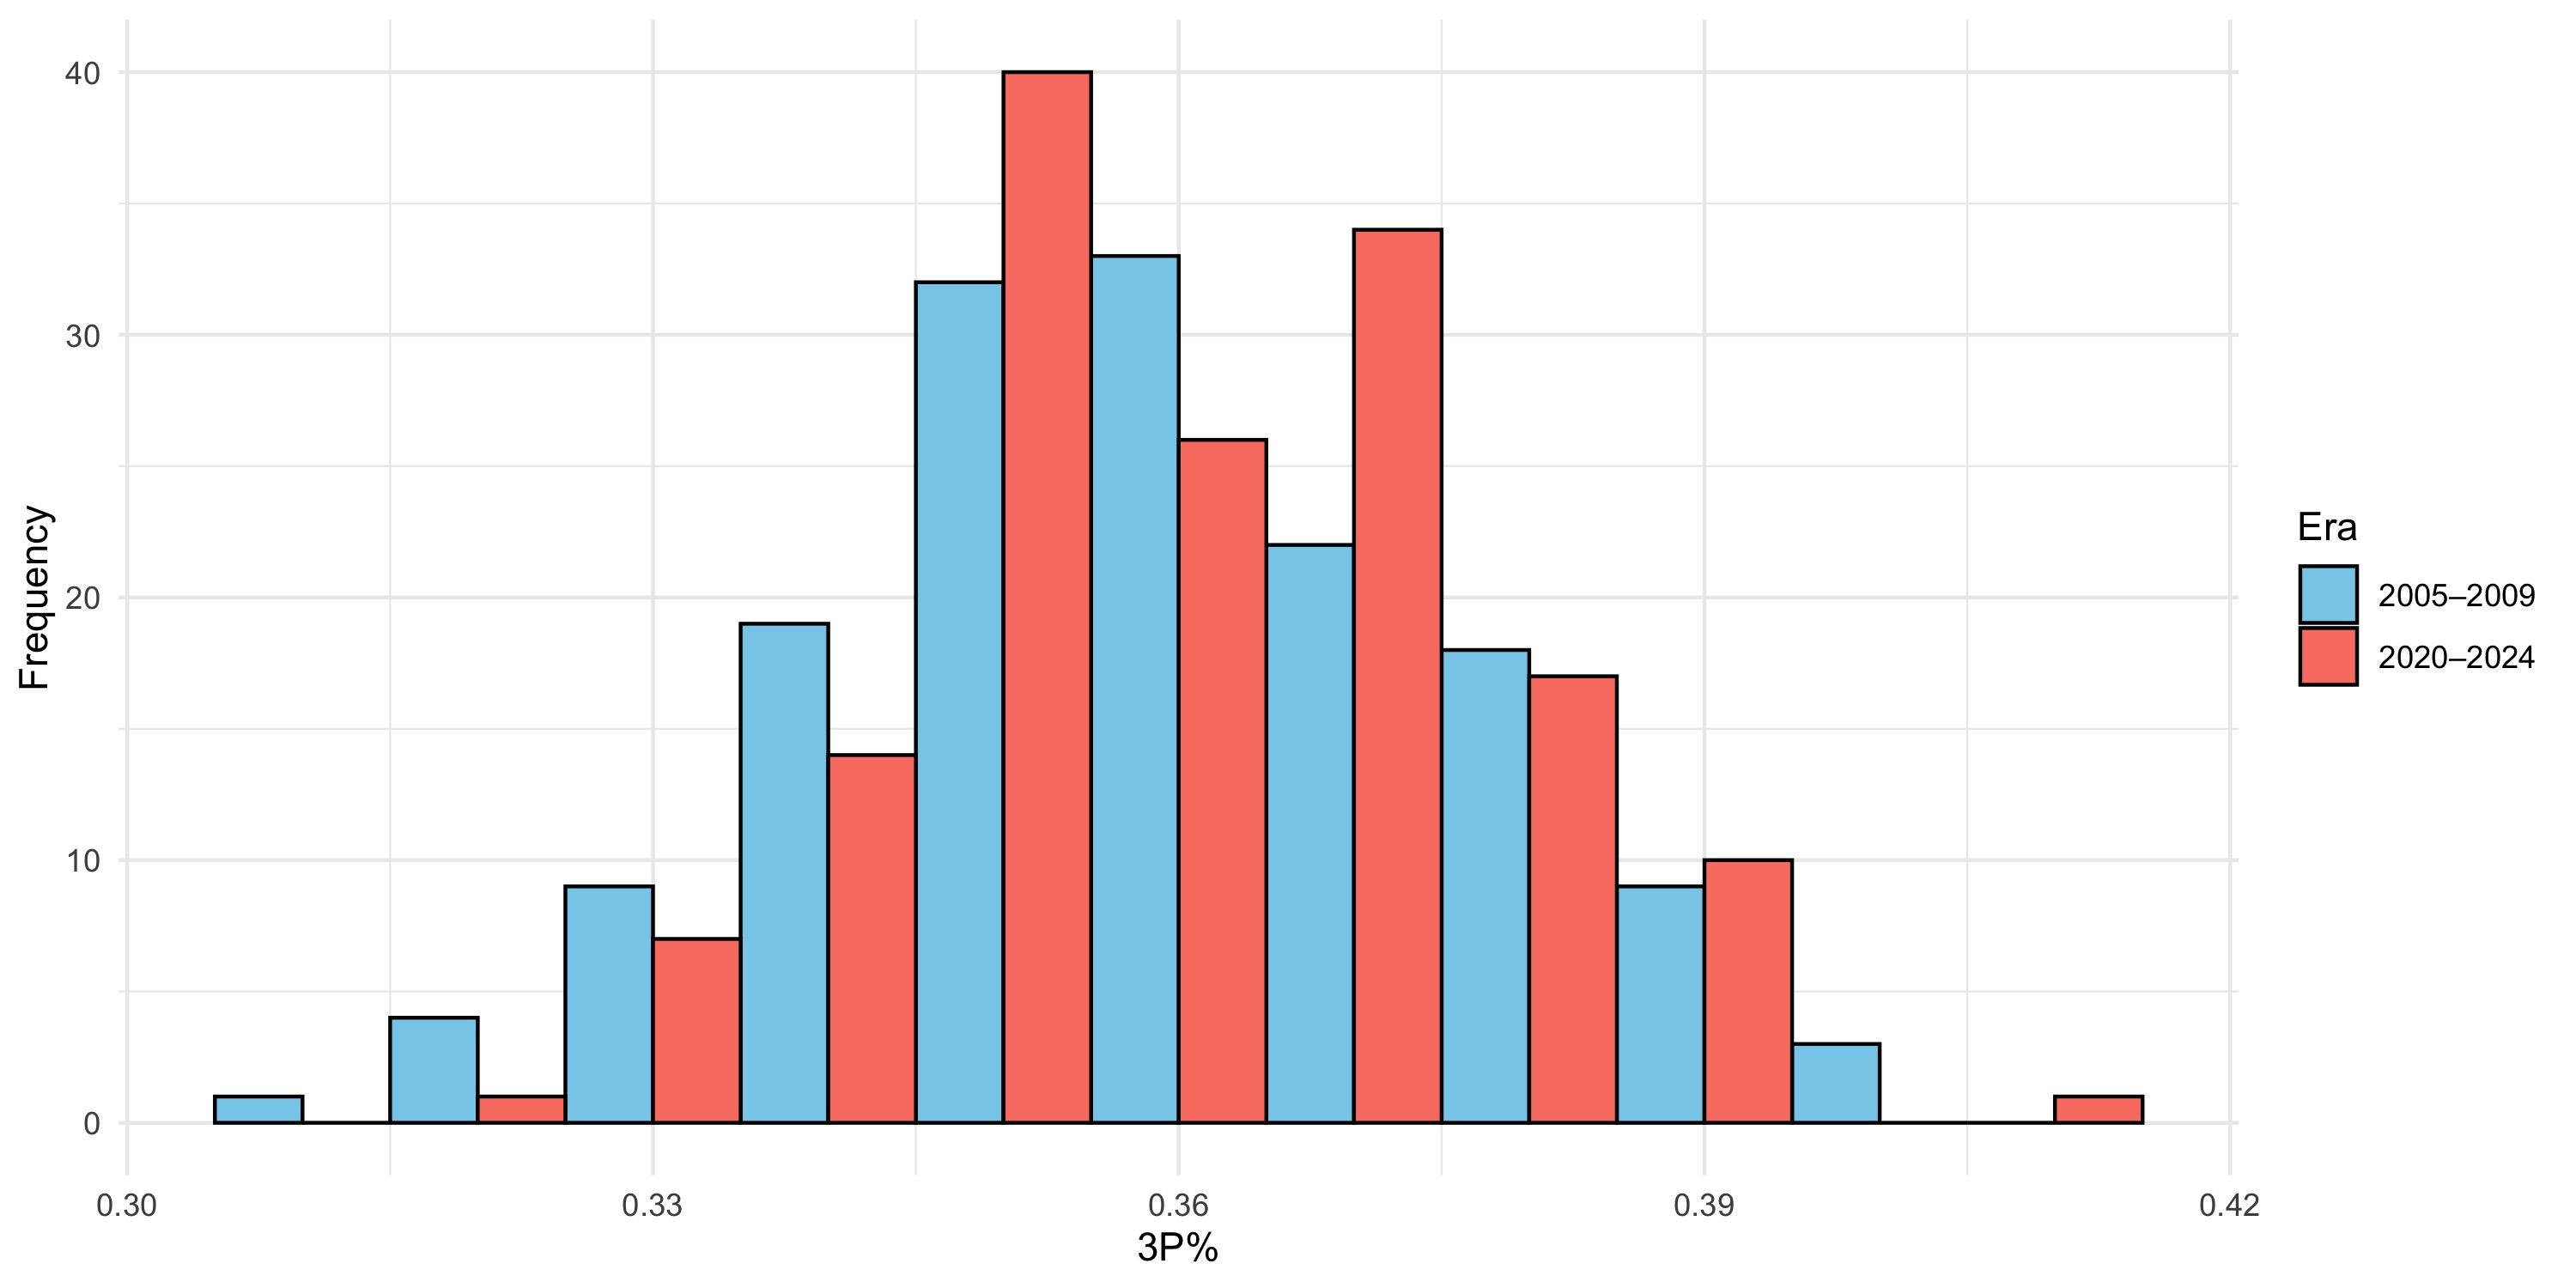
\includegraphics[width=0.6\textwidth]{figure/3 point shooting percentage.jpg}
    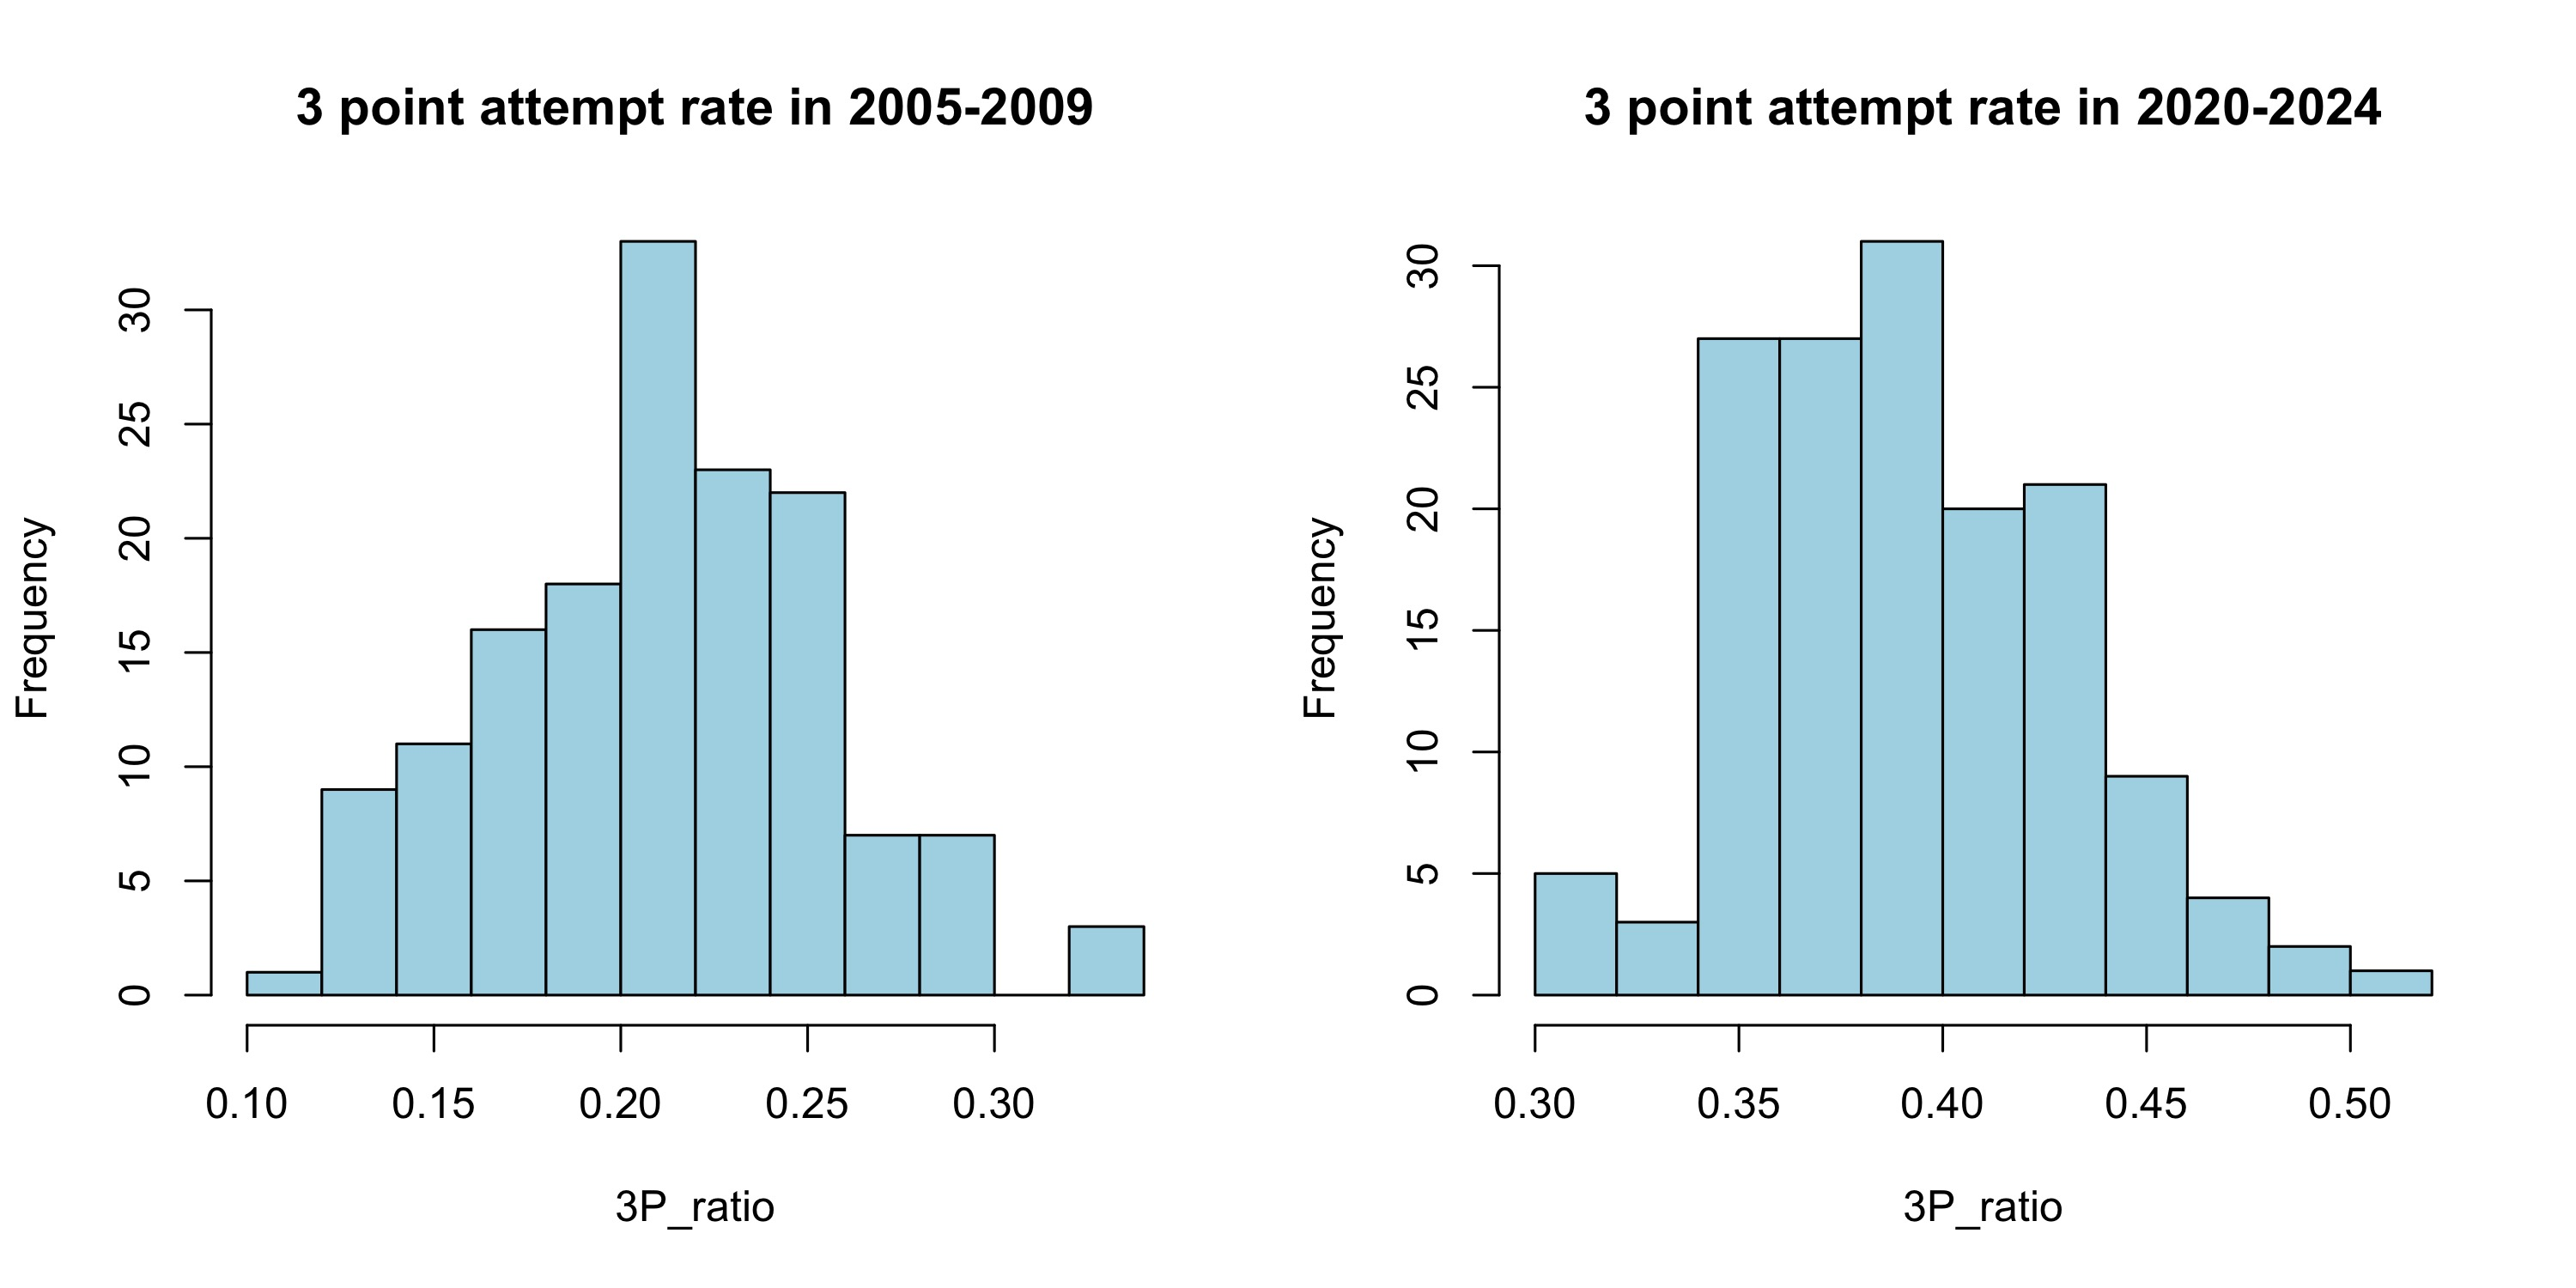
\includegraphics[width=0.6\textwidth]{figure/3 point attempt rate.jpg}
    \caption{Changes in three-point attempt rate (left) and shooting accuracy (right) between 2005-2009 and 2020-2024.}
    \label{fig:1}
\end{figure}

% The second set of histograms(Figure \ref{fig:3P_attempt_rate}) displays the three-point attempt rate (3P\_ratio), defined as the proportion of a team's total field goal 
% attempts that are three-pointers. We observe a substantial rightward shift over time: in the 2005–2009 period, teams clustered around a 
% 20\% attempt rate, whereas by 2020-2024, the distribution centers around 38-40\%. This sharp increase visually confirms the commonly 
% cited notion that the NBA has entered a “small ball” era, characterized by greater reliance on perimeter shooting and faster-paced offenses.


% Together, these visualizations provide structural evidence for a fundamental change in league-wide offensive strategy. 
% The sharp increase in three-point attempt rates, coupled with stable or slightly improved three-point accuracy, sets the stage for our 
% central analysis: evaluating whether and how the growing emphasis on three-point shooting translates into higher win rates in the modern NBA.
Figure \ref{fig:1} provides a visual summary of the changes in three-point shooting behavior over time. The pie charts (left) show a 
substantial increase in the proportion of field goal attempts that are three-pointers, rising from 21.1\% in 2005-2009 to 39.2\% 
in 2020-2024. Meanwhile, the overlaid histograms indicate that teams have also become slightly more accurate, 
with the distribution of three-point shooting percentages shifting modestly to the right in the modern era. This actually a very strong 
signal since the accuracy is kind of hard to improve, such a notable shift is already very impressive.

These visual trends motivate our modeling approach: to statistically examine whether the growing reliance on three-point shooting 
has translated into greater influence on win rate, and whether this shift reflects a broader structural transformation in NBA 
offensive strategy.


\subsection{Data Preprocess}
Our data preprocessing involved two main steps. First, we retrieved the raw team-level statistics using the NBA API, 
where each table corresponds to a single season, and each row records a team's aggregate performance for that year. 
We combined the annual tables into four period-specific datasets, grouped by five-year intervals (2005-2009, 2010-2014, 2015-2019, 
and 2020-2024).

Second, we performed variable selection and transformation. A large portion of the original variables were rankings (e.g., team 
rank in field goal percentage or rebounds), which we excluded, as they are ordinal and not suitable for regression analysis. 
We also observed that while the raw data included a few basic statistics (e.g., win percentage and FG3\_PCT), it lacked several 
metrics relevant to our analysis. We therefore manually computed key variables, including win rate (WinRate), three-point attempt 
rate (3P\_ratio), three-point shooting percentage (3P\%), and two-point shooting percentage (2P\%). Since 3P\_ratio and 2P\_ratio 
are linearly dependent (they sum to 1), we included only 3P\_ratio in our models to avoid multicollinearity.

\subsection{Statistical Techniques}
We began our analysis by fitting a simple linear regression model using team-level three-point field goal percentage (3P\%), 
two-point field goal percentage (2P\%), and three-point attempt rate (3P\_ratio) to predict regular season win rate. This baseline 
model allowed us to examine how different aspects of team shooting efficiency are associated with success across seasons.

To assess whether the impact of three-point shooting has changed over time, we then fit an interactive linear model. In this model, 
we included interaction terms between the shooting variables and a binary era indicator (early era vs. modern era). This design 
enables us to statistically test whether the relationship between three-point efficiency and win rate has become significantly 
stronger in recent years, rather than relying solely on visual or descriptive comparisons.

% Finally, to account for potential confounding factors, we extended our model by including a set of additional control variables 
% such as total rebounds, turnovers, free throw percentage, and assists. These variables may influence team success and could also 
% be correlated with shooting performance, thus serving as potential confounders. Including them in the model allows us to assess 
% whether the effect of three-point shooting remains significant after accounting for other team performance metrics.

To investigate the influence of potential confounding variables, we expanded our interactive model by incorporating a range of 
other team statistics that could plausibly affect win rates. These included measures such as free throw percentage 
(\texttt{FT\_PCT}), offensive and defensive rebounds (\texttt{OREB}, \texttt{DREB}).

To evaluate the validity of our regression models, we also performed standard diagnostic checks. Specifically, we examined 
residual plots including Residuals vs Fitted, Normal Q-Q, Scale-Location, and Residuals vs Leverage. These plots allow us to 
assess key assumptions of linear regression such as linearity, homoscedasticity, normality of residuals, and the presence of 
influential points. The diagnostic results did not reveal major violations, suggesting that the fitted models are reasonably 
appropriate for the data.


%----------------------------------------------------------------------------------------
% Results Section
%----------------------------------------------------------------------------------------

\section{Results}
\subsection{Initial Analysis: Period-Specific Associations}
% Word Count: Approx. 350-450 words

To get a first look at how relationships might have changed, we fitted separate simple linear regression models for 
different 5-year periods, specified as follows:
\begin{equation*}
\text{WinRate} = \beta_0 + \beta_1 \times \text{3P\%} + \beta_2 \times \text{2P\%} + \beta_3 \times \text{3P\_ratio} + \epsilon
\end{equation*}
We focus here on comparing the earliest period with the latest period(2005-2009 vs 2020-2024). Figure \ref{fig:period_models} displays the summary outputs 
for these two models.

\begin{figure}[htbp] 
    \centering
    % Using subcaption package for side-by-side figures
    % Make sure \usepackage{subcaption} is in your preamble
    \begin{subfigure}{0.48\textwidth}
        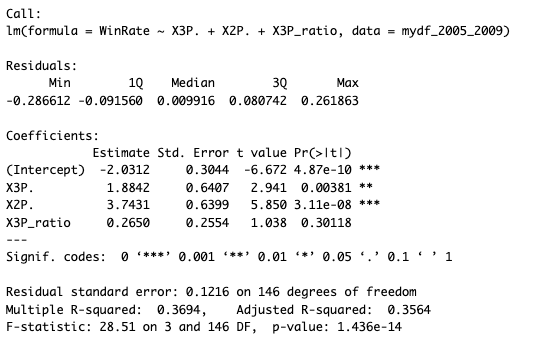
\includegraphics[width=\linewidth]{figure/model0_2005_2009.png} % Ensure path is correct
        \caption{Model Summary: 2005-2009 Period.}
        \label{fig:model_0509}
    \end{subfigure}\hfill % \hfill creates space between figures
    \begin{subfigure}{0.48\textwidth}
        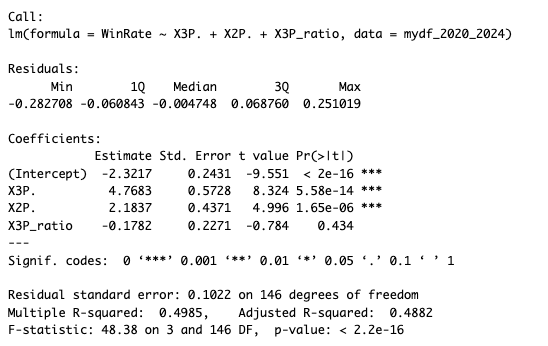
\includegraphics[width=\linewidth]{figure/model0_2020_2024.png} % Ensure path is correct
        \caption{Model Summary: 2020-2024 Period.}
        \label{fig:model_2024}
    \end{subfigure}
    \caption{Comparison of Parsimonious Linear Regression Model Summaries for Early and Recent Eras.}
    \label{fig:period_models}
\end{figure}

Comparing the outputs shown in Figure \ref{fig:period_models}, we observe notable differences between the two periods. 
In the 2005-2009 model (Figure \ref{fig:model_0509}), both two-point percentage (\texttt{X2P.}) and three-point percentage 
(\texttt{X3P.}) show statistically significant positive associations with \texttt{WinRate}. However, the estimated coefficient 
for \texttt{X2P.} (approximately 3.74) is considerably larger than that for \texttt{X3P.} (approximately 1.88). Furthermore, 
the p-value associated with \texttt{X2P.} is much smaller ($p < 0.001$) compared to the p-value for \texttt{X3P.} 
($p \approx 0.0038$). In this earlier period, the three-point attempt rate (\texttt{X3P\_ratio}) was not found to have 
a statistically significant association with \texttt{WinRate}.

In contrast, when looking at the 2020-2024 model (Figure \ref{fig:model_2024}), while both \texttt{X2P.} and \texttt{X3P.} 
remain statistically significant and positively associated with \texttt{WinRate}, their apparent relative importance seems to 
have reversed. The coefficient for \texttt{X3P.} (approximately 4.77) is now substantially larger than the coefficient 
for \texttt{X2P.} (approximately 2.18). The very small p-value for \texttt{X3P.} ($p < 0.001$) indicates a very strong 
statistical association in this recent period. Similar to the earlier period, \texttt{X3P\_ratio} remains non-significant. 
This initial comparison suggests a potential shift: the positive association between three-point efficiency and winning appears 
stronger in the recent era, while the association for two-point efficiency might have weakened.

To visualize these changes more broadly, we plotted the estimated coefficients and their corresponding p-values (on a reversed 
log scale) for \texttt{X3P.} and \texttt{X2P.} across four consecutive 5-year periods. Figure \ref{fig:trends} presents these trends.

% Figure for trend plots side-by-side
\begin{figure}[htbp] 
    \centering
    % Using subcaption package for side-by-side figures
    \begin{subfigure}{0.48\textwidth}
        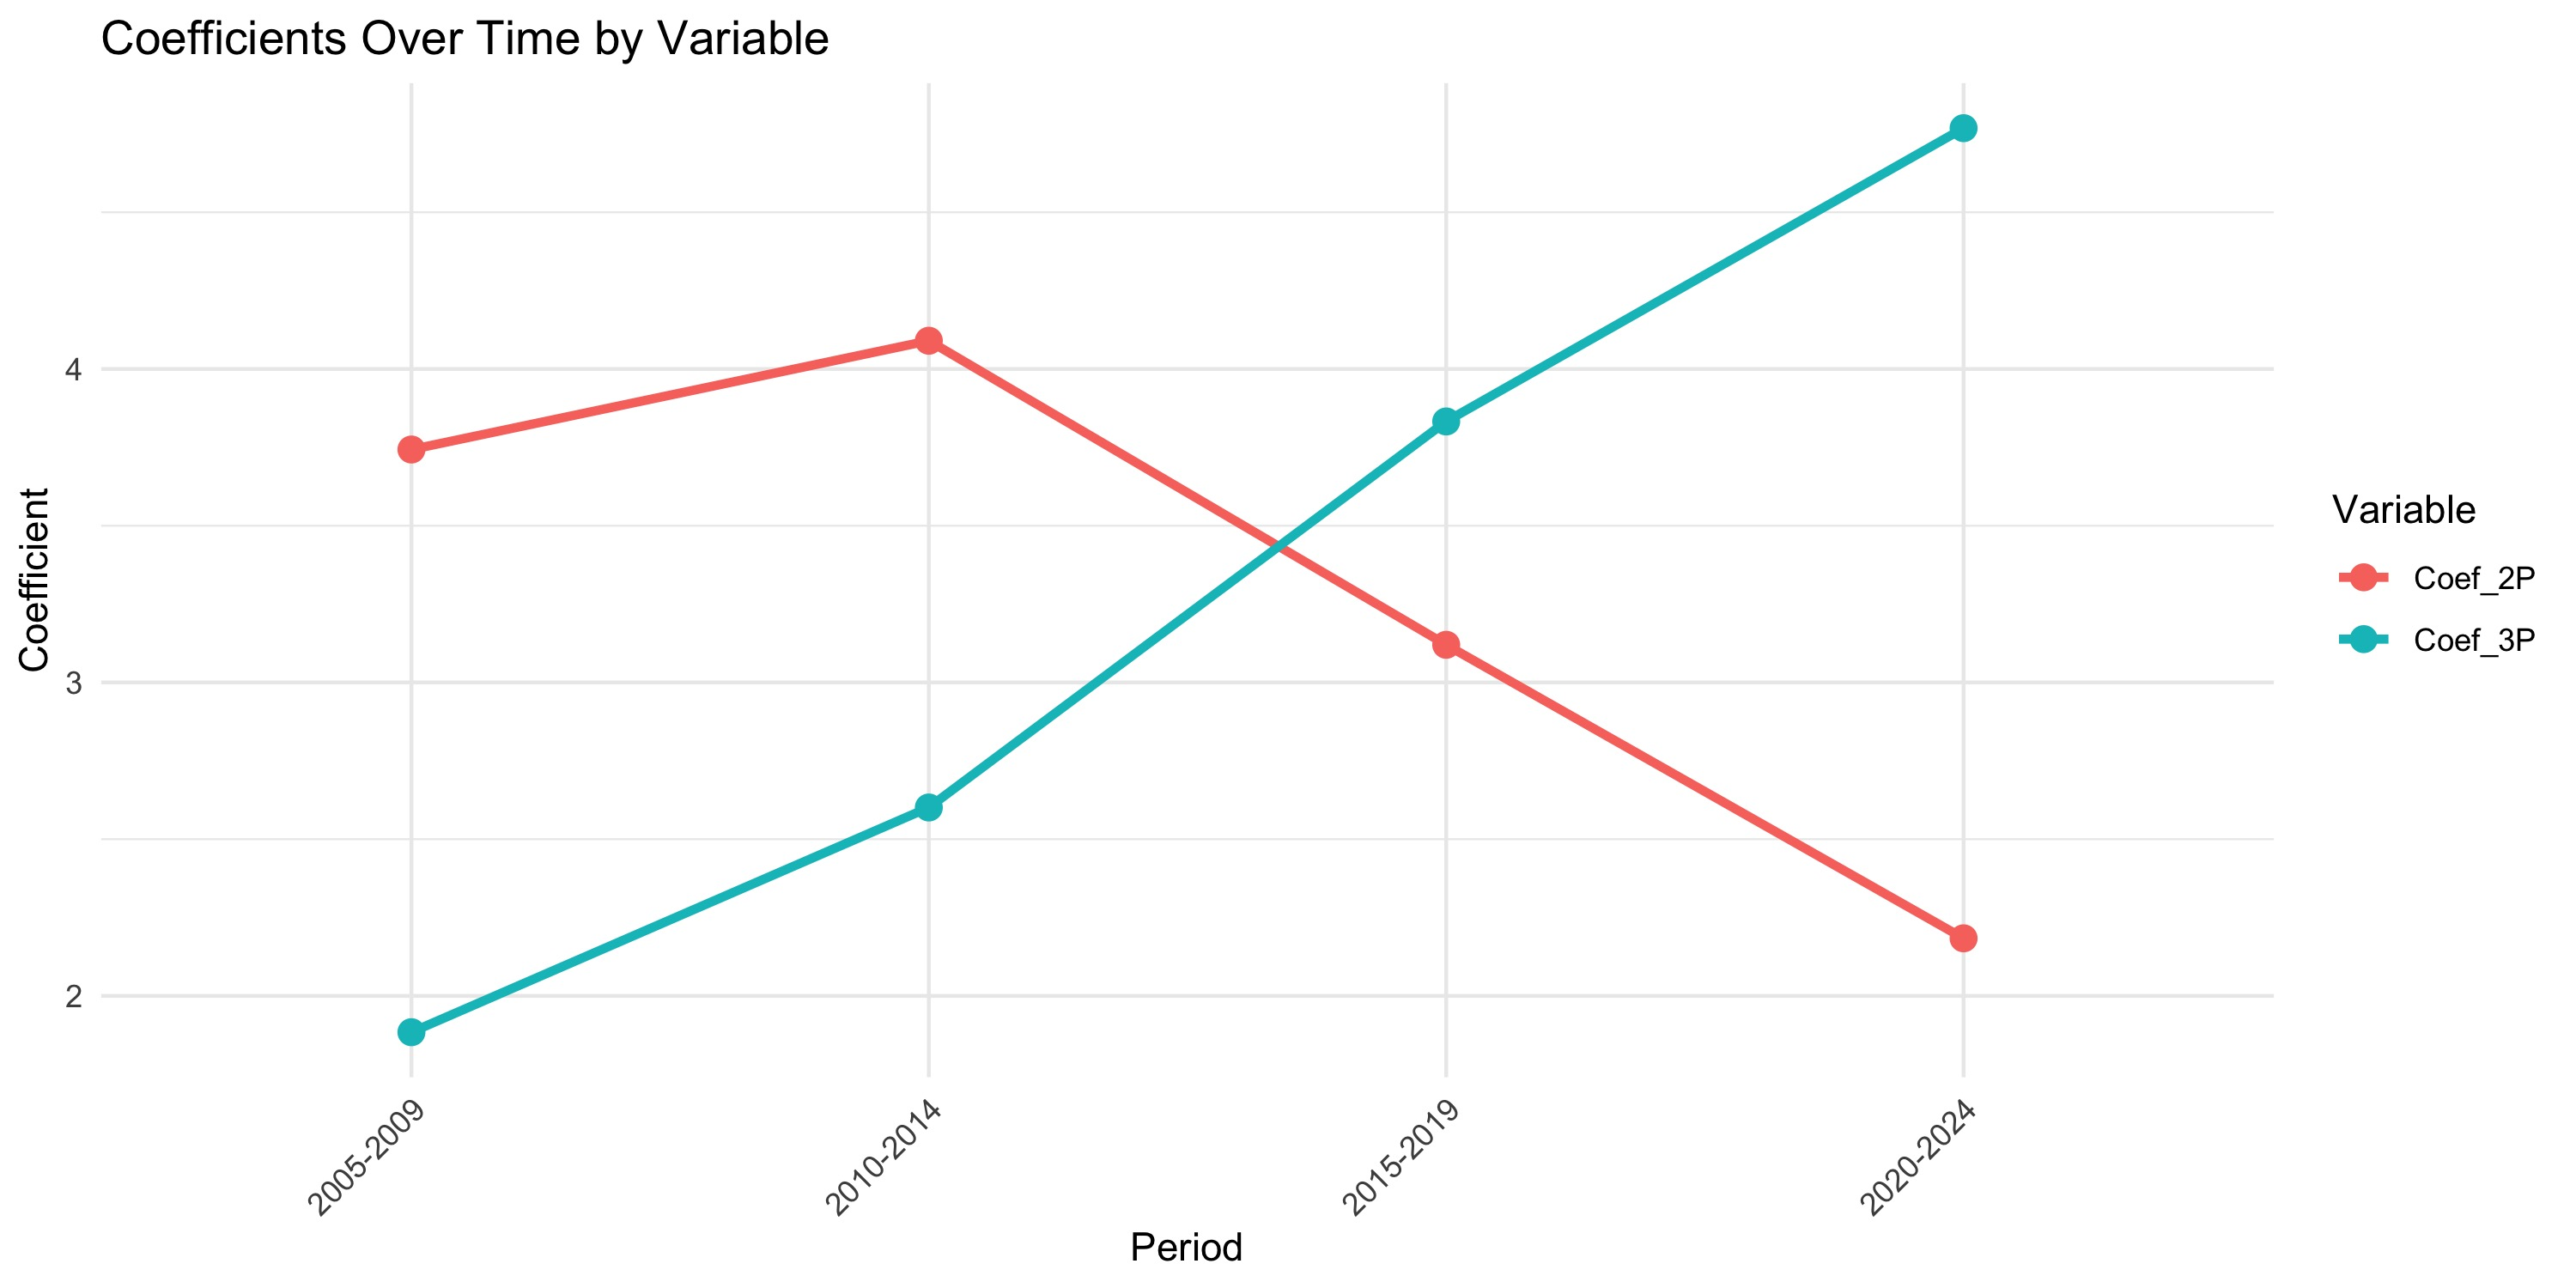
\includegraphics[width=\linewidth]{figure/Coefficients Over Time by Variable.jpg} % Ensure path is correct
        \caption{Trend in Estimated Coefficients.}
        \label{fig:coef_trends}
    \end{subfigure}\hfill
    \begin{subfigure}{0.48\textwidth}
        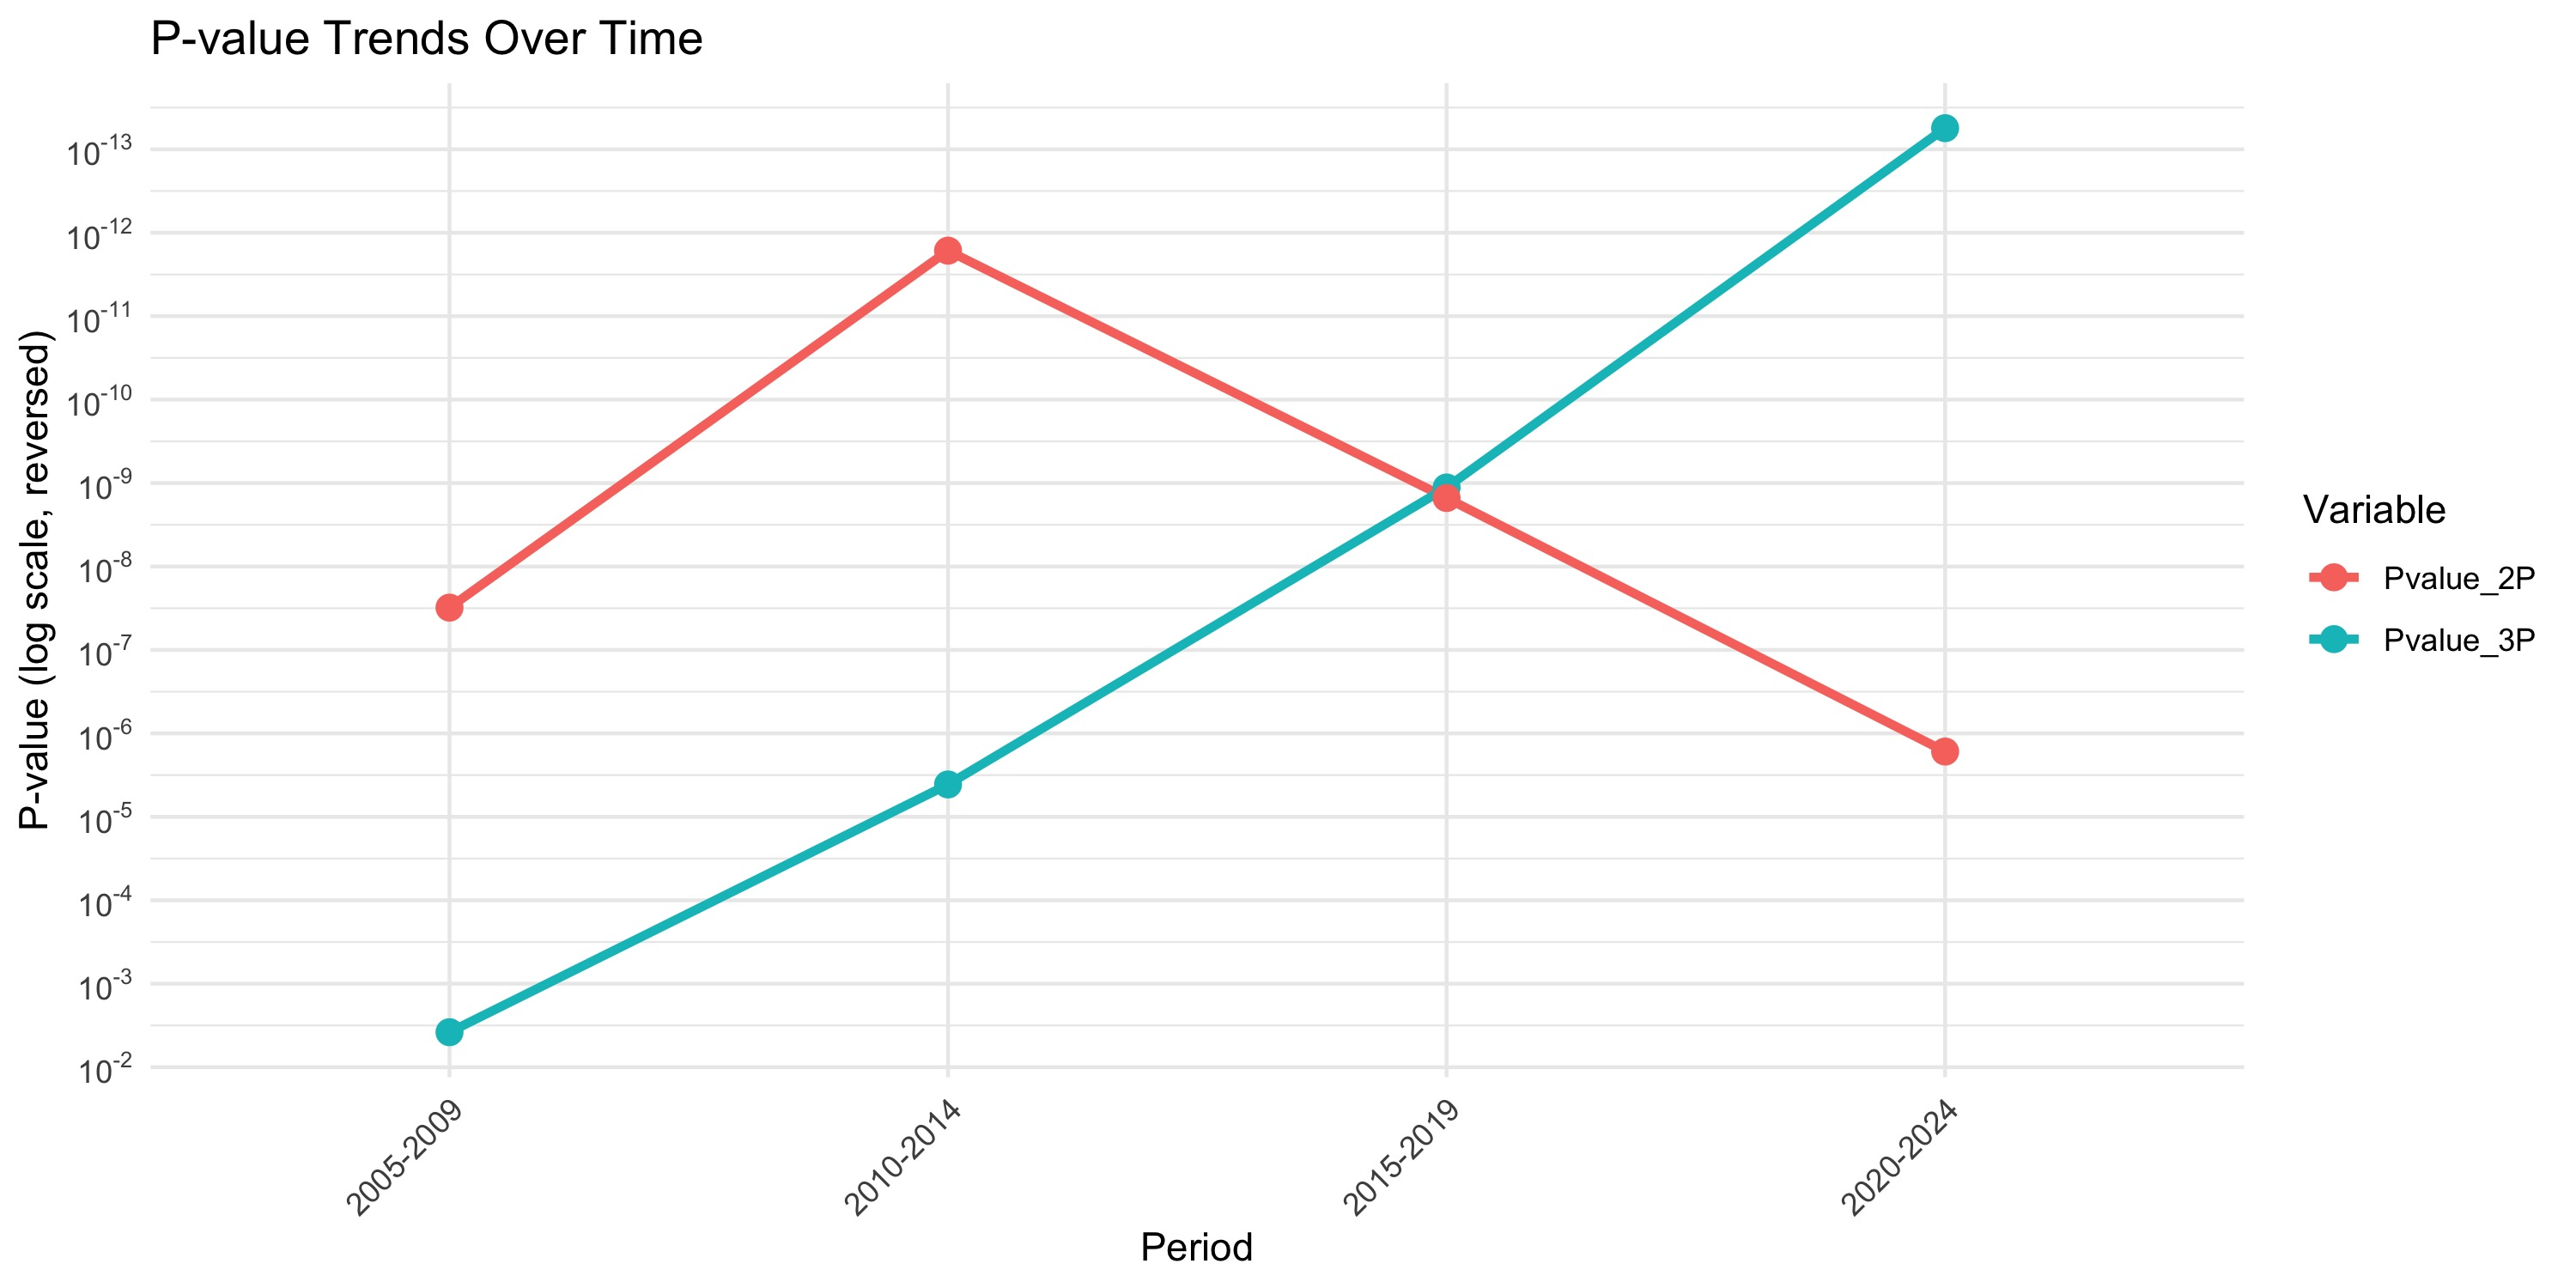
\includegraphics[width=\linewidth]{figure/P-value Trends Over Time.jpg} % Ensure path is correct
        \caption{Trend in P-values (Reversed Log Scale).}
        \label{fig:pval_trends}
    \end{subfigure}
    \caption{Trends in Coefficients and P-values for \texttt{X3P.} and \texttt{X2P.} from Period-Specific Regressions.}
    \label{fig:trends}
\end{figure}

Figure \ref{fig:coef_trends} clearly shows the coefficient for \texttt{X3P.} (blue line) steadily increasing over time, 
while the coefficient for \texttt{X2P.} (red line) generally decreases after the 2010-2014 period. Figure \ref{fig:pval_trends} 
complements this by showing the p-value associated with \texttt{X3P.} decreasing (indicating strengthening statistical significance), 
while the p-value for \texttt{X2P.}, although remaining significant, shows less of a strengthening trend. These descriptive trends 
strongly indicate a changing relationship and motivate the use of an interaction model to formally test the significance of 
this observed shift.

\subsection{The Interaction Model}
% Word Count: Approx. 250-350 words

To capture the evolving relationship between shooting metrics and team success over time, we fit an interactive linear regression model incorporating both main effects and interaction terms with era. The model is specified as:
\begin{align*}
    \text{WinRate} =\ & \beta_0 + \beta_1 \cdot \text{3P\%} + \beta_2 \cdot \text{2P\%} + \beta_3 \cdot \text{3P}_{\text{ratio}} + \beta_4 \cdot \text{2P}_{\text{ratio}} + \beta_5 \cdot \text{Era} \\
    & + \beta_6 \cdot (\text{3P\%} \times \text{Era}) + \beta_7 \cdot (\text{2P\%} \times \text{Era}) + \beta_8 \cdot (\text{3P}_{\text{ratio}} \times \text{Era}) \\
    & + \beta_9 \cdot (\text{2P}_{\text{ratio}} \times \text{Era}) + \epsilon
    \end{align*}

Our model summary is shown in Table \ref{tab:interaction_summary_R}.

% --- START: Interaction Model Summary Table based on R output image ---
\begin{table}[htbp]
\centering
\caption{Summary of Interaction Model Results (Response: WinRate, based on R output)}
\label{tab:interaction_summary_R}
% Using booktabs package for better table formatting
% Make sure \usepackage{booktabs} is in your preamble
\begin{tabular}{lrrrl}
\toprule
Predictor & Estimate & Std. Error & t value & Pr(>|t|) \\
\midrule
(Intercept) & -2.0312 & 0.2812 & -7.224 & 4.41e-12 *** \\ 
X3P. & 1.8842 & 0.5918 & 3.184 & 0.001610 ** \\ 
X2P. & 3.7431 & 0.5910 & 6.334 & 9.02e-10 *** \\ 
X3P\_ratio & 0.2650 & 0.2359 & 1.123 & 0.262187 \\ 
Era (1 = 2020-24) & -0.2905 & 0.3879 & -0.749 & 0.454448 \\ 
\textbf{X3P.:Era} & \textbf{2.8842} & \textbf{0.8641} & \textbf{3.338} & \textbf{0.000954 ***} \\ 
X2P.:Era & -1.5594 & 0.7616 & -2.047 & 0.041509 * \\ 
X3P\_ratio:Era & -0.4431 & 0.3434 & -1.290 & 0.197976 \\ 
\midrule
\multicolumn{5}{l}{\textit{Signif. codes: 0 `***' 0.001 `**' 0.01 `*' 0.05 `.' 0.1 ` ' 1}} \\
\multicolumn{5}{l}{Residual standard error: 0.1123 on 292 degrees of freedom} \\ 
\multicolumn{5}{l}{Multiple R-squared: 0.4301, Adj. R-squared: 0.4165} \\ 
\multicolumn{5}{l}{F-statistic: 31.49 on 7 and 292 DF, p-value: < 2.2e-16} \\ 
\bottomrule
\end{tabular}
\end{table}
% --- END: Interaction Model Summary Table ---

The results in Table \ref{tab:interaction_summary_R} provide the crucial statistical evidence for our study. 
The key term is the interaction between three-point percentage and era (\texttt{X3P.:Era}). Its coefficient is 
approximately 2.8842 and is highly statistically significant (p $\approx$ 0.000954, `***'). This positive and 
significant interaction term statistically confirms our central hypothesis: the positive association between a 
team's \texttt{X3P.} and its \texttt{WinRate} is significantly stronger in the 2020-2024 era (Era=1) compared to 
the baseline 2005-2009 era (Era=0). Specifically, for every one percentage point increase in \texttt{X3P.}, the 
associated increase in \texttt{WinRate} is estimated to be about 2.88 points higher in the 2020-2024 era than it 
was in the 2005-2009 era, holding other predictors constant.

Furthermore, the interaction term \texttt{X2P.:Era} has a coefficient of approximately -1.5594 and is statistically 
significant at the 0.05 level (p $\approx$ 0.0415, `*'). This suggests that the positive association between \texttt{X2P.} 
and \texttt{WinRate} significantly weakened in the later era compared to the baseline era. These findings align perfectly 
with the descriptive trends shown in Figure \ref{fig:coef_trends}. The main effects for \texttt{X3P.} and \texttt{X2P.} 
represent their associations in the baseline (2005-2009) era, both being positive and significant. Other terms, including 
\texttt{X3P\_ratio}, its interaction with era, and the main effect of \texttt{Era}, did not show statistically significant 
associations in this model. The overall model provides a reasonable fit (Adjusted R-squared $\approx$ 0.4165) and is 
highly significant overall (F-statistic p-value < 2.2e-16). The strong significance of the \texttt{X3P.:Era} interaction 
provides the formal statistical validation for our thesis about the changing relationship.

\subsection{Consideration of Confounders}
In our primary analysis, we aim to understand the statistical association between three-point shooting --- particularly 
three-point percentage (\texttt{3P\%}) --- and team win rates (\texttt{WinRate}). However, various other aspects of team 
performance might be associated with both a team's reliance on three-point shooting and its overall success, potentially 
confounding the observed relationship between our primary variables. Understanding and accounting for these potential confounders 
is important for interpreting the association more clearly.

To address this, we considered including a range of basketball performance metrics as control variables (potential confounders) 
in our modeling. These included metrics related to other aspects of scoring efficiency, ball control, and defense, such as free 
throw percentage (\texttt{FT\_PCT}), offensive and defensive rebounds (\texttt{OREB}, \texttt{DREB}), turnovers (\texttt{TOV}), 
steals (\texttt{STL}), blocks (\texttt{BLK}), and fouls committed or drawn (\texttt{PF}, \texttt{PFD}).

These variables were considered because they represent critical facets of overall team performance beyond just shooting percentages. 
It is plausible that these factors correlate with both shooting behavior and win rates. For example, teams that secure more 
defensive rebounds (\texttt{DREB}) or generate more steals (\texttt{STL}) might create more fast-break or transition opportunities, 
potentially leading to different types or qualities of three-point attempts. Similarly, teams committing fewer 
turnovers (\texttt{TOV}) or drawing more fouls (\texttt{PFD}) might represent more disciplined or skilled teams overall, 
which could correlate independently with both higher win rates and specific offensive strategies (including three-point efficiency).

By including such variables in the regression model(see Appendix Figure \ref{fig:confounder_model_appendix} for details), the goal is to statistically adjust for their association with both the 
predictors and the outcome. This approach helps to isolate the independent statistical association of the primary shooting 
metrics (\texttt{3P\%}, \texttt{2P\%}, etc.) with team success (\texttt{WinRate}), allowing for a more nuanced interpretation 
of the relationship after accounting for these other performance dimensions. (As noted in the Results section, key findings 
regarding \texttt{3P\%} remained significant after including controls in exploratory models).


\subsection{Model Diagnostics}
\begin{figure}[htbp] 
    \centering
    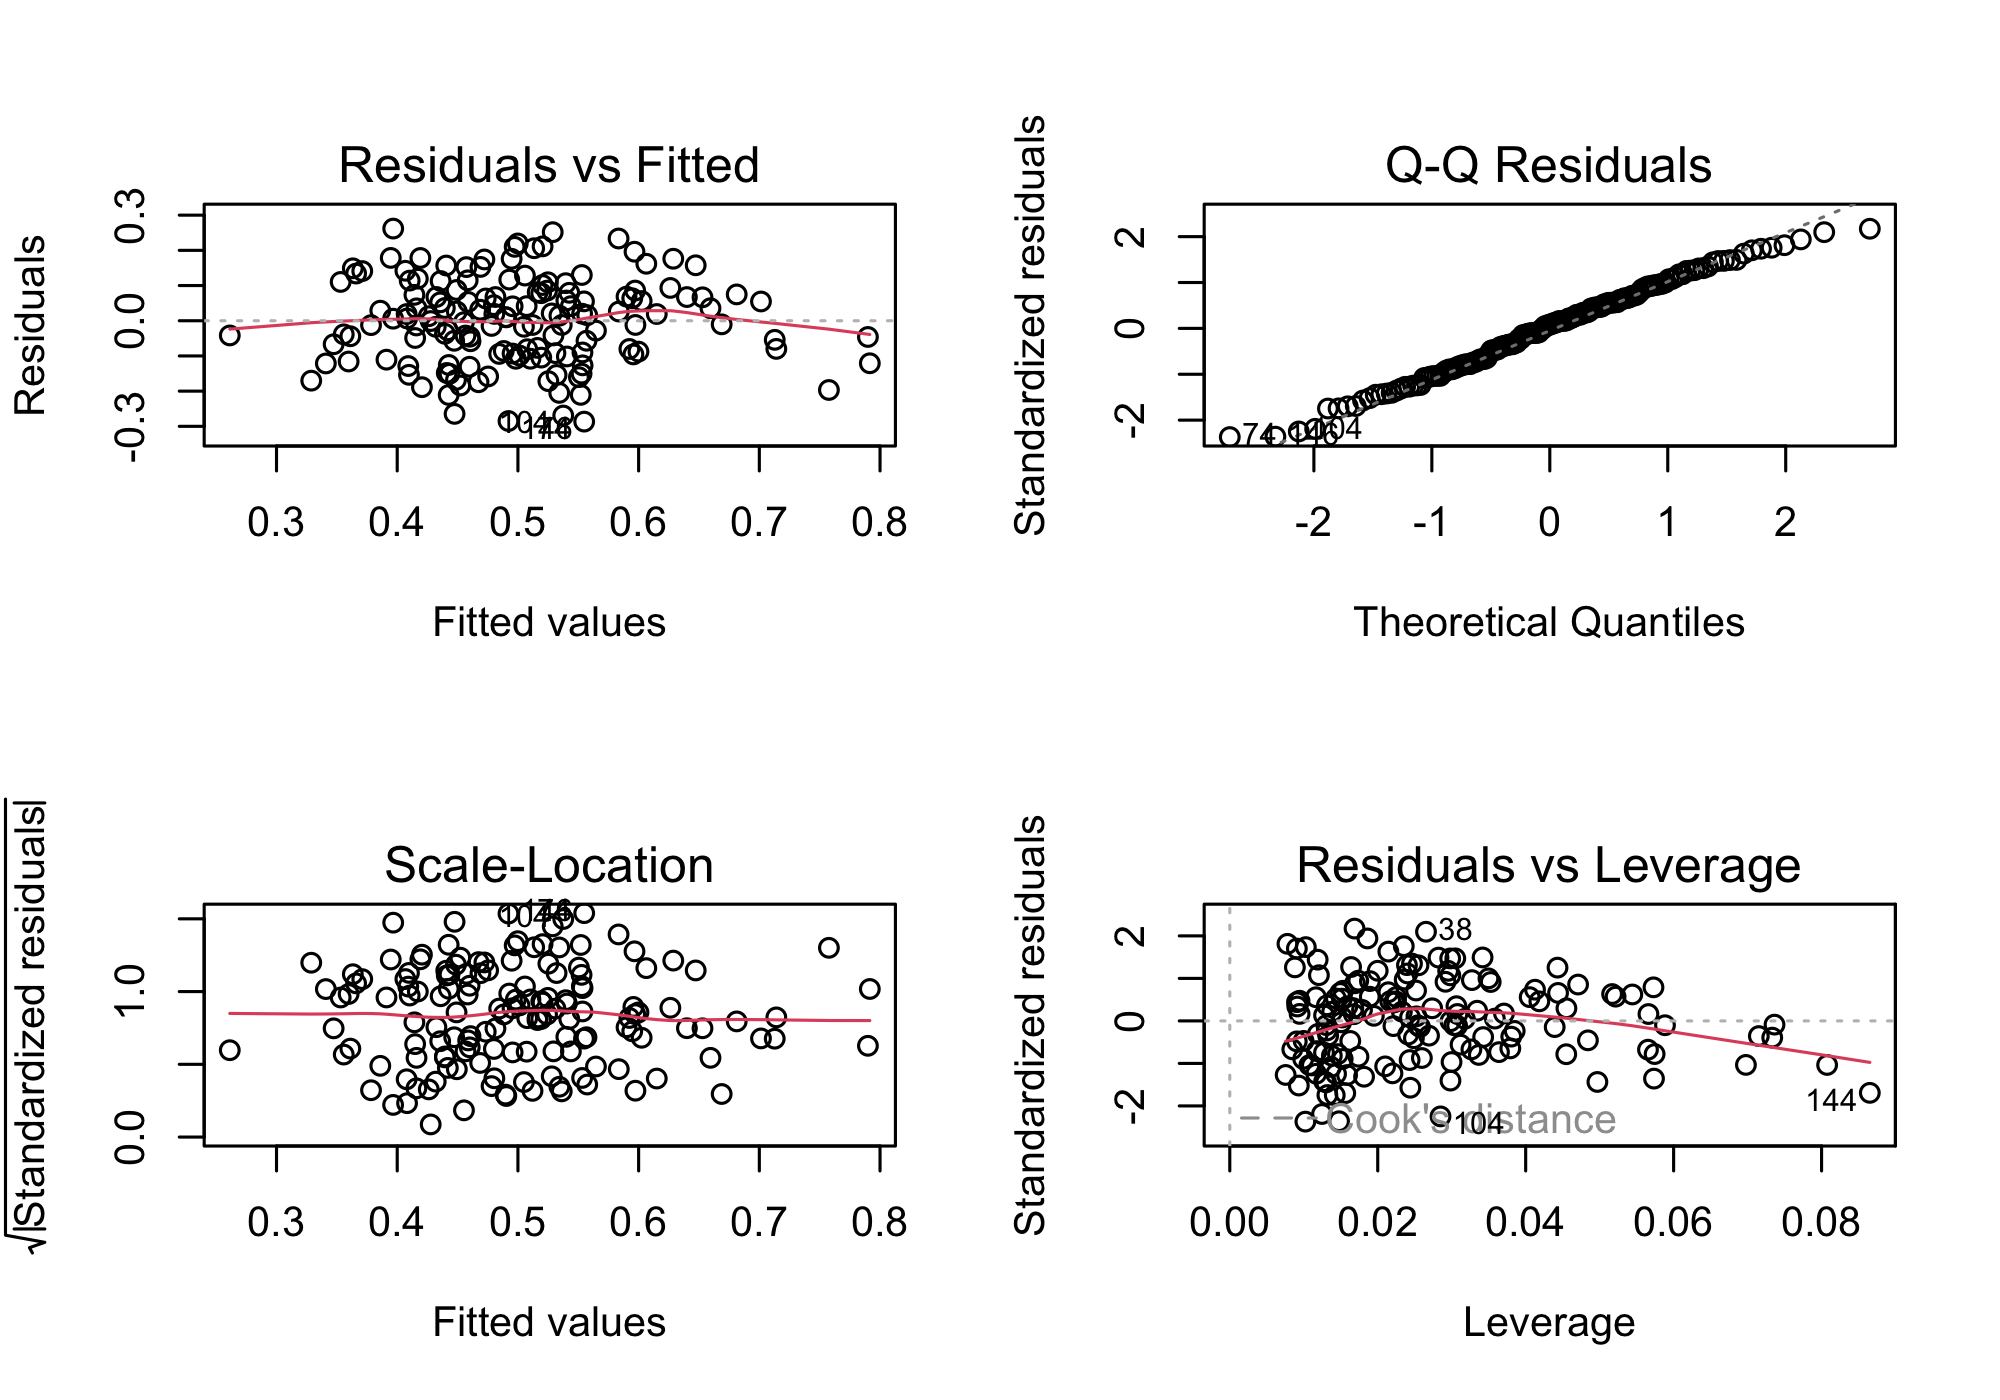
\includegraphics[width=0.9\textwidth]{figure/diagnostic_plots_mydf_2005_2009.png} 
    \caption{Diagnostic Plots for the Interaction Model.} 
    \label{fig:diagnostic_plots_interaction}
\end{figure}
\FloatBarrier %
Finally, we assessed the validity of the assumptions underlying the OLS regression for our final interaction model (results in Table \ref{tab:interaction_summary_R}). The standard diagnostic plots associated with this model are presented in Figure \ref{fig:diagnostic_plots_interaction}. 

Visual inspection of these plots provides confidence in our model. The 'Residuals vs Fitted' plot displays points scattered fairly randomly around the horizontal line at zero, without a clear non-linear pattern or a distinct funnel shape, which supports the assumptions of linearity and constant variance (homoscedasticity). The 'Normal Q-Q' plot shows the standardized residuals falling generally close to the theoretical diagonal line, suggesting that the normality assumption for the residuals is reasonably met, although there might be slight deviations in the tails as is common with real-world data. The 'Scale-Location' plot further examines the homoscedasticity assumption; the points appear relatively evenly spread across the range of fitted values, and the smoothed red line is mostly flat, providing additional support for constant variance. Lastly, the 'Residuals vs Leverage' plot helps identify potentially influential observations. Most points exhibit low leverage. While point 144 shows slightly higher leverage than others, its standardized residual does not appear extreme, and no points seem to significantly exceed typical Cook's distance thresholds (though contours are not explicitly labeled). Therefore, based on this visual assessment, the standard OLS assumptions seem adequately satisfied for our interaction model, lending validity to the statistical inferences we have drawn from it.


%----------------------------------------------------------------------------------------
% End of Results Section
%----------------------------------------------------------------------------------------

%----------------------------------------------------------------------------------------
% Conclusion Section (Revised Word Count: Approx. 350-400 words)
%----------------------------------------------------------------------------------------

\section{Conclusion} % Main Section Title

\subsection{Summary of Findings and Implications} % Sub-section 4.1
% Word Count: Approx. 180-200 words

This project statistically investigated the perceived emergence of a "Three-Point Era" in the NBA by analyzing how the relationship 
between shooting efficiency and team success evolved over time. Using data from the 2005–2009 and 2020–2024 NBA regular seasons 
(source: NBA API), we examined the association between three-point percentage (\texttt{3P\%}) and team win rate (\texttt{WinRate}), 
controlling for two-point efficiency and shot selection ratios. Our regression results show that while three-point efficiency was 
not significantly associated with win rate in the earlier period, it became a statistically significant predictor of success in the 
modern era. The key supporting evidence is the statistically significant interaction term between era and three-point percentage 
(\texttt{Era:X3P.}) in our model (see Table~\ref{tab:interaction_summary_R}), which indicates that the strength of this association 
increased by approximately 2.88 units in the 2020–2024 period compared to 2005–2009. This provides compelling quantitative support 
for the claim that the strategic value of three-point shooting has risen over time. Although our observational design cannot 
establish causality, the magnitude and significance of the shift strongly align with the notion that efficient three-point 
shooting has become a more decisive factor in team success under modern league dynamics.

\subsection{Limitations of the Analysis} % Sub-section 4.3
% Word Count: Approx. 120-150 words
Several limitations must be considered when interpreting these results. Primarily, as this study relies on observational data, 
we cannot make definitive causal claims. The observed associations, and the changes in them, could be influenced by numerous 
unobserved confounding variables that evolved alongside shooting strategies. Potential confounders include changes in defensive 
rules and strategies over the years, the overall evolution of player skill sets (especially the rise of prolific shooters), 
influential coaching philosophies adapting to or driving trends, the impact of specific superstar players on their teams' style 
and success, uncaptured variations in team defense quality, or even factors like player injuries or strength of schedule within 
specific seasons. While our model controls for key efficiency and shot selection metrics, it cannot account for all such complex, 
potentially time-varying confounders. Other limitations include the specific choice of time periods for comparison and the inherent 
assumptions of the linear regression model framework.

\subsection{Future Research} % Sub-section 4.4
% Word Count: Approx. 30-40 words
Future research could aim to address these limitations by incorporating data on defensive metrics, coaching changes, or player-level statistics if available. Exploring different time frames or using panel data methods might also provide further insights. Applying more advanced methods aimed at causal inference from observational data could be valuable, though potentially challenging.

%----------------------------------------------------------------------------------------
% End of Conclusion Section
%----------------------------------------------------------------------------------------
%----------------------------------------------------------------------------------------
% References
%----------------------------------------------------------------------------------------

% \newpage % Includes a new page
% \pagenumbering{roman} % Changes page numbering to roman page numbers
% %\bibliography{literature}

% \bibliography{literature.bib} % Add the filename of your bibliography
% \bibliographystyle{apsr} % Defines your bibliography style

%----------------------------------------------------------------------------------------
% Appendix
%----------------------------------------------------------------------------------------

\newpage
\pagenumbering{roman} % Changes page numbering to roman page numbers

\section*{Appendix}

\begin{figure}[htbp] % Figure environment to place the image
    \centering % Center the image
    % Make sure the path 'figure/image_eaa7f2.png' is correct relative to your .tex file
    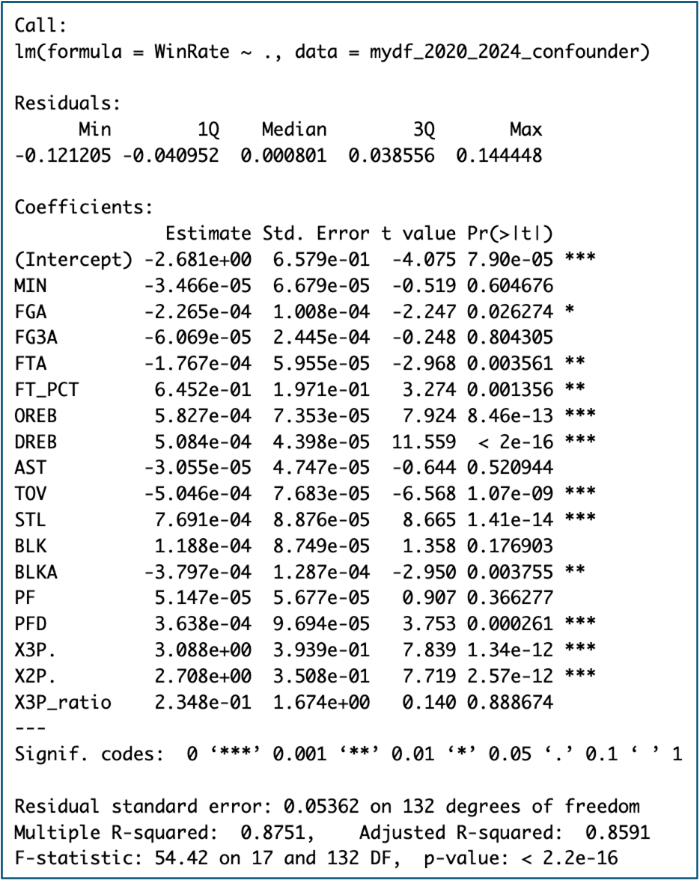
\includegraphics[width=0.8\textwidth]{figure/confounder_model_appendix.png} 
    \caption{Example Regression Model Output Including Confounding Variables (Data: 2020-2024 Period). This model includes variables such as $FT_PCT$, OREB, DREB, TOV, STL, BLK, PF, PFD etc., in addition to the primary shooting metrics.}
    \label{fig:confounder_model_appendix} % Label for referencing this figure
\end{figure}
% For citing, please see this sheet: http://merkel.texture.rocks/Latex/natbib.php

% %----------------------------------------------------------------------------------------
% % Appendix
% %----------------------------------------------------------------------------------------
% \newpage % Includes a new page
% \section*{Appendix} % Stars disable section numbers
% % \appendix % Uncomment if you want to add an "automatic" appendix
% \pagenumbering{Roman} % Changes page numbering to Roman page numbers

% \blindtext % Adds some blind text

% %----------------------------------------------------------------------------------------
% % Declaration
% %----------------------------------------------------------------------------------------
% \newpage % Includes a page break
% \thispagestyle{empty} % Leaves the page style empty (no page number, no header, no footer)
% \section*{Statutory Declaration} % Stars disable section numbers

% \begin{otherlanguage}{german}
% Hiermit versichere ich, dass diese Arbeit von mir pers\"{o}nlich verfasst ist und dass ich keinerlei fremde Hilfe in Anspruch genommen habe. Ebenso versichere ich, dass diese Arbeit oder Teile daraus weder von mir selbst noch von anderen als Leistungsnachweise andernorts eingereicht wurden. W\"{o}rtliche oder sinngem\"{a}{\ss}e \"{U}bernahmen aus anderen Schriften und Ver\"{o}ffentlichungen in gedruckter oder elektronischer Form sind gekennzeichnet. S\"{a}mtliche Sekund\"{a}rliteratur und sonstige Quellen sind nachgewiesen und in der Bibliographie aufgef\"{u}hrt. Das Gleiche gilt f\"{u}r graphische Darstellungen und Bilder sowie f\"{u}r alle Internet-Quellen. Ich bin ferner damit einverstanden, dass meine Arbeit zum Zwecke eines Plagiatsabgleichs in elektronischer Form anonymisiert versendet und gespeichert werden kann. Mir ist bekannt, dass von der Korrektur der Arbeit abgesehen und die Pr\"{u}fungsleistung mit nicht ausreichend bewertet werden kann, wenn die Erkl\"{a}rung nicht erteilt wird.
% \end{otherlanguage}

% \vspace*{1in} % Adds extra space between two paragraphs

% \noindent I hereby declare that the paper presented is my own work and that I have not called upon the help of a third party. In addition, I affirm that neither I nor anybody else has submitted this paper or parts of it to obtain credits elsewhere before. I have clearly marked and acknowledged all quotations or references that have been taken from the works of others. All secondary literature and other sources are marked and listed in the bibliography. The same applies to all charts, diagrams and illustrations as well as to all Internet resources. Moreover, I consent to my paper being electronically stored and sent anonymously in order to be checked for plagiarism. I am aware that the paper cannot be evaluated and may be graded ``failed'' (``nicht ausreichend'') if the declaration is not made.\\

% %\vspace*{1in} % Adds extra space

% % Add field for signature, date, and place
% \hfill \signature{} 


% %---------------------------------------------------------------------------------

\end{document}
